\documentclass[conference]{IEEEtran}
\usepackage{cite}
\usepackage{amsmath,amssymb,amsfonts}
\usepackage{algorithmic}
\usepackage{graphicx}
\graphicspath{{../}{./}}
\usepackage{textcomp}
\usepackage{xcolor}
\usepackage{booktabs}
\usepackage{multirow}
\usepackage{url}
\usepackage{subcaption}

\def\BibTeX{{\rm B\kern-.05em{\sc i\kern-.025em b}\kern-.08em
    T\kern-.1667em\lower.7ex\hbox{E}\kern-.125emX}}

\begin{document}

\title{Drug Integrity Algebra: Quantifying End-to-End\\Pharmaceutical Safety with Subjective Logic}

\author{\IEEEauthorblockN{Muntaser Syed\IEEEauthorrefmark{1}, Mahasen Enam\IEEEauthorrefmark{2}, Nidadavolu Venkat Durga Sai Siva Vara Prasad Raju\IEEEauthorrefmark{3}, and Marius Silaghi\IEEEauthorrefmark{1}}
\IEEEauthorblockA{\IEEEauthorrefmark{1}Florida Institute of Technology, Melbourne, FL, USA\\
msyed2011@my.fit.edu, msilaghi@fit.edu}
\IEEEauthorblockA{\IEEEauthorrefmark{2}Independent Researcher, UAE\\
maha.enam@gmail.com}
\IEEEauthorblockA{\IEEEauthorrefmark{3}Birla Institute of Technology and Science, Pilani, India\\
2018ht13247@wilp.bits-pilani.ac.in}
}

\maketitle

\begin{abstract}
Pharmaceutical supply chains protect patient safety through serialization
and cold chain monitoring, yet current systems like the UAE's Tatmeen,
the US Drug Supply Chain Security Act, and the EU Falsified Medicines
Directive rely on binary pass/fail thresholds that discard continuous
evidence, ignore measurement uncertainty, and evaluate each node in
isolation. We present a drug integrity algebra grounded in J\o sang's
Subjective Logic that maps five heterogeneous evidence types at each
supply chain node to opinions with explicit belief, disbelief, and
uncertainty components, fuses them within nodes via cumulative fusion,
and propagates them across a directed acyclic graph using the deduction
operator with causal conditionals. In Monte Carlo evaluation across
seven failure scenarios, three pharmaceutical product categories, and
five comparison methods (including a Dempster-Shafer baseline), the
algebra matches the rule-based baseline on detection and localization
(DR=1.000, LA=1.000) while providing what that baseline discards: graded
severity scores that rank failure severity with statistical significance
(Spearman $\rho$=0.976, $p$=3.3$\times$10$^{-5}$), the only method to do
so, and explicit uncertainty that localizes the affected evidence type
and node. In the noiseless regime the algebra detects 1\% counterfeit
infiltration where weighted scoring requires 10\% and Bayesian inference
over 5\%; under benign operational noise, fixed thresholds of any kind
fail, and detection of subtle failures becomes a question of evidence
volume, which we quantify. Ablation identifies per-dimension opinion
monitoring as the critical architectural component, and the
Dempster-Shafer baseline demonstrates both conflict normalization and
evidence dilution, producing zero bits of Shannon entropy across all
failure conditions.
\end{abstract}

\begin{IEEEkeywords}
subjective logic, pharmaceutical supply chain, drug integrity,
uncertainty quantification, evidence fusion, cold chain monitoring
\end{IEEEkeywords}

%===================================================================
\section{Introduction}
%===================================================================

The World Health Organization estimates that one in ten medical products
circulating in low- and middle-income countries is substandard or
falsified, with global expenditure on such products reaching
US\$30.5 billion annually~\cite{who2024sf}. In 2022 alone, contaminated
cough syrups caused the deaths of over 300 children across the Gambia,
Indonesia, and Uzbekistan~\cite{who2023cough}. Regulatory responses
have produced national track-and-trace mandates: the UAE's Tatmeen
platform (Ministerial Decree No.~73/2021)~\cite{tatmeen_decree73},
the US Drug Supply Chain Security Act (DSCSA)~\cite{dscsa2013}, and the
EU Falsified Medicines Directive~\cite{eufmd2011}. These systems
require serialization of individual packages using GS1 DataMatrix
codes and verification at each custody transfer.

All three systems share a fundamental architectural limitation: they
operate on binary pass/fail thresholds at each supply chain node
independently. This design has three consequences that directly affect
patient safety.

First, thresholds destroy continuous evidence. A temperature reading of
7.9\textdegree C and one of 2.1\textdegree C both produce ``pass'' on a
2-8\textdegree C product, but carry different risk signals. A facility
scanning 100\% of packages and one scanning 10\% generate identical
``compliant'' status if all scanned items pass, despite an order-of-magnitude
difference in verification confidence.

Second, no existing system quantifies the uncertainty in its own
assessments. When a pharmacy receives a batch rated ``compliant,'' the
system provides no indication of whether that rating rests on thorough
evidence or sparse observations.

Third, each node reports independently. There is no mechanism to compose
evidence across the supply chain into an end-to-end integrity assessment
at the point of dispensing.

We address all three limitations with a \textit{drug integrity algebra}
grounded in J\o sang's Subjective Logic (SL)~\cite{josang2016}. The
algebra defines five evidence-to-opinion formation functions that map
serialization scans, cold chain readings, shelf life status,
documentation completeness, and recall status to SL opinions with
explicit belief, disbelief, and uncertainty. These opinions fuse within
each node via cumulative fusion and propagate across the supply chain
directed acyclic graph (DAG) using the deduction operator with causal
conditionals that reflect the physical irreversibility of drug
compromise.

Our contributions are:
\begin{enumerate}
\item A formal mapping of five pharmaceutical evidence types to SL
      opinions, using only established operators from J\o sang's
      textbook, with the application-specific evidence encodings stated
      as explicit modeling assumptions.
\item A supply chain DAG model grounded in the UAE Tatmeen system's
      EPCIS event architecture and Ministerial Decree No.~73/2021.
\item A chain-level integrity algebra using deduction-based cross-node
      propagation, justified by the irreversibility of drug compromise.
\item Empirical evaluation across seven failure scenarios, three product
      categories, and five comparison methods including a
      Dempster-Shafer baseline.
\item Identification of per-dimension opinion monitoring as the critical
      architectural component through systematic ablation.
\end{enumerate}

%===================================================================
\section{Background and Related Work}
%===================================================================

\subsection{Track-and-Trace Systems}

Pharmaceutical serialization mandates require unique identifiers on
each saleable unit and verification at custody transfers. The UAE's
Tatmeen system, operated by EVOTEQ under the Ministry of Health and
Prevention, mandates four GS1 DataMatrix elements per package: GTIN,
batch number, expiry date, and serial number (Article~5, Ministerial
Decree No.~73/2021)~\cite{tatmeen_decree73}. Both sender and receiver
must report each custody transfer as paired EPCIS events, and dispensing
verification at pharmacies is synchronous~\cite{tatmeen_dispenser_v3}.
The DSCSA~\cite{dscsa2013} and EU FMD~\cite{eufmd2011} impose similar
requirements with jurisdiction-specific variations. All three systems
produce binary verification outcomes. Our B1 baseline mirrors this
approach.

\subsection{Blockchain for Pharmaceutical Supply Chain}

Blockchain-based systems such as MediLedger~\cite{mediledger} and
TraceLink provide tamper-proof audit trails for custody transfer
records. Bocek et al.~\cite{bocek2017} integrated IoT temperature
sensors with Ethereum smart contracts for pharmaceutical cold chain
monitoring. These systems ensure the \textit{integrity of records} but
do not reason about what those records mean for drug safety. A
blockchain faithfully recording that 5\% of scan verifications failed
does not produce a risk assessment. Our algebra is complementary:
blockchain provides the data infrastructure, and the algebra reasons
over that data.

\subsection{IoT Cold Chain Monitoring}

Real-time temperature monitoring with IoT sensors and machine learning
anomaly detection has received substantial attention. Gillespie et
al.~\cite{coldchain_iot2023} demonstrated real-time anomaly detection
in cold chain transportation using IoT technology, achieving improved
visibility and spoilage reduction. LSTM and ANN architectures have been
applied to predict temperature excursions before they occur. These
approaches monitor a single evidence dimension (temperature), require
training data, and do not produce calibrated uncertainty estimates or
compose assessments across supply chain nodes. Our cold chain evidence
type is one of five dimensions in the algebra.

\subsection{Dempster-Shafer Theory}

Dempster-Shafer theory (DST)~\cite{shafer1976} provides a framework for
combining evidence via mass functions and Dempster's rule of
combination. DST has been applied to fraud detection~\cite{ds_fraud2021}
and supplier selection~\cite{ds_supplier2017}. SL is sometimes
characterized as extending DST to address known
limitations~\cite{josang2016}: DST has no trust discounting operator for
propagating opinions through networks, is subject to Zadeh's
paradox~\cite{zadeh1984} when evidence sources conflict, lacks a base
rate for meaningful probability projection, and has no temporal decay
mechanism. Our evaluation includes a DST baseline (B4) that
demonstrates both conflict normalization and evidence dilution in the
pharmaceutical domain.

\subsection{Subjective Logic}

J\o sang's Subjective Logic~\cite{josang2016} extends probabilistic
logic with explicit uncertainty representation. An SL opinion
$\omega = (b, d, u, a)$ decomposes confidence into belief $b$,
disbelief $d$, and uncertainty $u$ (with $b + d + u = 1$), plus a base
rate $a$ for probability projection $P(\omega) = b + a \cdot u$. SL
has been applied to trust management in wireless mesh
networks~\cite{sl_manet2017}, to context-dependent trust decisions among
agents~\cite{sl_vanet2013}, and to e-commerce reputation~\cite{josang2016}. Multi-source fusion operations have been formalized by Van der Heijden et
al.~\cite{sl_multisource2018}. To our
knowledge, no prior work has applied SL to pharmaceutical supply chain
integrity assessment. This paper is the first to do so.

%===================================================================
\section{Drug Integrity Algebra}
%===================================================================

\subsection{Supply Chain DAG}

\textbf{Definition 1.} A pharmaceutical supply chain is a directed
acyclic graph $G = (N, E)$ where $N = \{n_1, \ldots, n_k\}$ are custody
nodes and $E \subseteq N \times N$ are custody transfer edges. Each node
$n_i$ has type $\tau(n_i) \in \{\textsc{manufacturer}, \textsc{importer},
\textsc{warehouse}, \textsc{distributor}, \textsc{pharmacy}\}$, and each
edge carries an EPCIS transfer record. A product path
$\pi = (n_1, \ldots, n_m)$ traces a batch from manufacture to
dispensing.

Our evaluation uses a five-node path grounded in the Tatmeen
architecture: manufacturer (overseas), importer (UAE), central warehouse,
distributor, and pharmacy.

\subsection{Evidence Taxonomy}

\textbf{Definition 2.} At each node $n_i$, five evidence types are
observable:
\begin{itemize}
\item \textbf{E1 - Serialization:} scan results per package (success,
      failure, unscanned).
\item \textbf{E2 - Cold chain:} temperature time-series with target
      range and sensor coverage.
\item \textbf{E3 - Shelf life:} remaining days relative to regulatory
      minimum.
\item \textbf{E4 - Documentation:} presence of required and critical
      documents (Certificate of Analysis, GMP Certificate, etc.).
\item \textbf{E5 - Recall status:} whether the batch is under active
      recall.
\end{itemize}

\subsection{Formation Functions}

\textbf{Definition 3.} Each evidence type maps to an SL opinion via a
formation function $\varphi_i$ using established SL operators.

\textbf{F1 (Serialization).} Given $s$ successful scans, $f$ failures,
and $N$ total packages, we apply \texttt{Opinion.from\_evidence}
(J\o sang \S3.4.3) with $r = s$, $w = f$, and prior weight $W$, then
apply trust discounting (J\o sang \S14.3) by the scan coverage ratio
$(s+f)/N$, so that unscanned packages appear as uncertainty rather than
as evidence.

\textbf{F2 (Cold chain).} Temperature readings produce positive evidence
(in-range readings) and negative evidence (excursions weighted by
severity), with sensor coverage modeled as a trust discount on the
resulting opinion.

\textbf{F3 (Shelf life).} The ratio $r = \text{remaining}/\text{minimum}$
maps to opinion via a piecewise linear function: at $r = 1.0$ (the
regulatory threshold), the opinion is vacuous, reflecting maximum
decision-relevant uncertainty.

\textbf{F4 (Documentation).} Document completeness maps to belief, with
critical documents (Certificate of Analysis, GMP Certificate) weighted
three times higher than routine documents.

\textbf{F5 (Recall).} An active recall produces a dogmatic disbelief
opinion $\omega = (0, 1, 0, a)$ that overrides all other evidence in
fusion. No recall produces a vacuous opinion, correctly encoding that
the absence of a recall is not evidence of safety.

All formation functions use only established operators from J\o sang's
textbook: the evidence-to-opinion mapping (\S3.4.3) and trust discounting
for sensor coverage (\S14.3). The encodings that feed those operators are
modeling assumptions of this work, not consequences of SL, and we state
them explicitly: the prior weight $W = 2/w_i$ with product-specific
weights $w_i$ between 0.6 and 1.6; base rates of 0.99 (serialization,
recall), 0.95 (cold chain), 0.90 (shelf life) and 0.80 (documentation);
a severity weight of $1 + \min(\Delta T / R,\, 5)$ per out-of-range
reading, $R$ being the range width; a shelf-life evidence scale of 10
per unit of $r$; a threefold weight for a missing critical document; the
compromised conditional $(0, 1, 0, 0.01)$, whose base rate is immaterial
because the opinion is dogmatic; and the detection rule, which flags a
chain when its projected probability falls below a calibrated threshold,
when any evidence dimension at any node has disbelief above 0.02 or
uncertainty above 0.50, or when chain-level uncertainty exceeds 0.30.
Section~\ref{sec:noise} reports how the results move when these are
varied.

\subsection{Within-Node Fusion}

\textbf{Definition 4.} At each node $n_i$, the five evidence opinions
fuse into a node-level integrity opinion via cumulative fusion
(J\o sang \S12.3):

\begin{equation}
\omega_{node}(n_i) = \bigoplus_{j=1}^{5} \varphi_j(\mathbf{e}_j^{(i)})
\label{eq:node_fusion}
\end{equation}

\noindent where $\bigoplus$ denotes cumulative fusion and
$\mathbf{e}_j^{(i)}$ is the evidence of type $j$ at node $i$.
Product-specific evidence weights are implemented by adjusting the
Dirichlet prior weight $W$ in each formation function, which controls
the opinion's dogmaticism in fusion without violating the
$b + d + u = 1$ constraint.

\subsection{Cross-Node Propagation}

\textbf{Definition 5.} Along a product path $\pi = (n_1, \ldots, n_m)$,
chain-level integrity is computed via the deduction operator (J\o sang
\S9.4) with causal conditionals:

\begin{equation}
\omega_{chain} = \omega_{n_1} \circledcirc (\omega_{n_2} \circledcirc (\cdots \circledcirc \omega_{n_m}))
\label{eq:chain_propagation}
\end{equation}

\noindent where $\circledcirc$ denotes deduction with conditional
opinions $\omega_{Y|x} = \omega_{remaining}$ (if upstream is safe) and
$\omega_{Y|\overline{x}} = (0, 1, 0, 0.01)$ (if upstream is
compromised).

The choice of deduction over trust discounting (\S14.3) is semantically
motivated. Trust discounting maps upstream disbelief to downstream
\textit{uncertainty}, which would mean ``we are uncertain about
downstream integrity because we distrust the upstream node.'' But drug
compromise is physically irreversible: a contaminated batch arriving at
a downstream node remains contaminated regardless of that node's
processes. Deduction with the conditional
$\omega_{Y|\overline{x}} = (0, 1, 0, 0.01)$ correctly maps upstream
disbelief to downstream \textit{disbelief}, preserving the causal
semantics.

\subsection{Properties}

The algebra satisfies five properties derived from SL's formal
guarantees.
\textbf{P1 (Monotonicity):} Additional positive evidence can only
increase chain belief or decrease uncertainty.
\textbf{P2 (Compositionality):} Chain opinion decomposes into
independently modifiable node opinions.
\textbf{P3 (Sensitivity):} Chain opinion responds proportionally to
evidence strength, with no threshold discontinuities.
\textbf{P4 (Uncertainty conservation):} Missing evidence produces
quantifiable uncertainty rather than silent pass or fail.
\textbf{P5 (Override):} Active recall produces chain-level disbelief
regardless of all other evidence.

%===================================================================
\section{Evaluation}
%===================================================================

\subsection{Setup}

We simulate a five-node supply chain path (manufacturer, importer,
central warehouse, distributor, pharmacy) grounded in the Tatmeen
architecture. Three product categories are evaluated: insulin
(refrigerated biologic, 2-8\textdegree C), amoxicillin tablets
(controlled room temperature, 15-25\textdegree C), and mRNA-based
therapy (frozen, -15 to -25\textdegree C). Normal operation generates
95-100\% scan rates with no scan failures (a nominal failure rate below
0.1\% rounds to zero at 100 packages), product-specific Gaussian
temperature noise ($\sigma$ = 0.8 to 1.5\textdegree C) clipped inside
the range, and complete documentation. Seven
failure scenarios (Table~\ref{tab:scenarios}) inject specific
compromises at designated nodes. Each configuration runs 1000 Monte
Carlo trials (seed 42, reproducible). Detection thresholds for the four
graded methods are calibrated at the 1st percentile of each method's
Normal-operation score distribution, targeting a 1\% false positive rate;
B1's binary output is thresholded at 0.5. Realized false positive rates on
1000 Normal trials are 0.010 for the SL algebra and B3 and 0.000 for B1,
B2 and B4. Detection rate (DR) is the fraction of trials flagged.
Localization accuracy (LA) is the fraction of flagged trials in which the
flagged node set contains a node where a failure was injected (for the
baselines, in which the lowest-scoring node is such a node); F7 injects
at two nodes and credits either. With 1000 trials per configuration,
DR=1.000 carries a 95\% Clopper-Pearson interval of [0.996, 1.000], the
widest interval on any reported rate is B3 on F3 (0.461, [0.430, 0.492]),
and the 95\% intervals on the mean scores in Table~\ref{tab:main_results}
are within $\pm 0.002$.

\begin{table}[t]
\centering
\caption{Failure Scenarios}
\label{tab:scenarios}
\footnotesize
\begin{tabular}{@{}lll@{}}
\toprule
ID & Description & Target Node \\
\midrule
F1 & Mild temp excursion (+2\textdegree C, 5\% readings) & Distributor \\
F2 & Severe temp excursion (+17\textdegree C, 50\%) & Distributor \\
F3 & Counterfeit insertion (5\% packages) & Importer \\
F4 & Scan omission (20\% scan rate) & Warehouse \\
F5 & Expired batch (50\% of regulatory min) & Distributor \\
F6 & Missing Certificate of Analysis & Importer \\
F7 & Cascading (F1 at warehouse + F4 at distributor) & Both \\
\bottomrule
\end{tabular}
\end{table}

\subsection{Comparison Methods}

Five methods are compared: the proposed SL algebra, a rule-based
threshold system (B1, mirroring Tatmeen), a weighted scoring approach
(B2), Bayesian probabilistic fusion (B3), and Dempster-Shafer evidence
theory (B4). B1 applies binary pass/fail checks per evidence type with
AND-aggregation across the chain. B2 computes continuous scores per type
with weighted averaging per node and weakest-link across the chain. B3
uses Beta-binomial conjugate posteriors per evidence type with
product-of-probabilities across nodes. B4 maps each evidence type to a
mass function over $\{safe, compromised\}$, combines within-node via
Dempster's rule, and combines cross-node via iterated Dempster's rule,
using the pignistic probability as its integrity score.

\subsection{Detection and Severity}

Table~\ref{tab:main_results} presents detection rates and severity
scores. The SL algebra achieves DR=1.000 and LA=1.000 across all 21
scenario-product combinations, as does the rule-based baseline B1; B2, B3
and B4 do not. Detection of these injected failures is therefore not what
separates the methods; the graded scores are.

\begin{table}[t]
\centering
\caption{Detection Rate and Mean Integrity Score (Insulin)}
\label{tab:main_results}
\footnotesize
\begin{tabular}{@{}l ccccc@{}}
\toprule
& SL & B1 & B2 & B3 & B4 \\
\midrule
\multicolumn{6}{@{}l}{\textit{Detection Rate}} \\
F1 mild    & 1.000 & 1.000 & 0.892 & 0.739 & 0.043 \\
F2 severe  & 1.000 & 1.000 & 1.000 & 1.000 & 0.129 \\
F3 counterfeit & 1.000 & 1.000 & 0.000 & 0.461 & 0.013 \\
F4 scan    & 1.000 & 1.000 & 1.000 & 1.000 & 0.010 \\
F5 expired & 1.000 & 1.000 & 1.000 & 1.000 & 0.000 \\
F6 CoA     & 1.000 & 1.000 & 1.000 & 1.000 & 0.048 \\
F7 cascade & 1.000 & 1.000 & 1.000 & 1.000 & 0.060 \\
\midrule
\multicolumn{6}{@{}l}{\textit{Mean Integrity Score}} \\
Normal     & 0.997 & 1.000 & 0.990 & 0.842 & 1.000 \\
F1 mild    & 0.951 & 0.000 & 0.981 & 0.800 & 1.000 \\
F2 severe  & 0.332 & 0.000 & 0.869 & 0.425 & 1.000 \\
\bottomrule
\end{tabular}
\end{table}

B2 completely misses 5\% counterfeit infiltration (F3, DR=0.000) because
the resulting node score (0.9875) equals its calibrated threshold and
never falls below it. B3 detects F3 at only 46\% because its
Beta-binomial posterior for 5\% counterfeiting sits near the calibrated
threshold. B1 detects everything but outputs 0.0 for all failures
regardless of severity, providing no information to the dispensing
pharmacist beyond a binary flag.

The severity scores in Table~\ref{tab:main_results} (bottom) reveal the
key qualitative difference. The SL algebra assigns $P(\omega) = 0.951$
to a mild excursion and $P(\omega) = 0.332$ to a severe one, correctly
reflecting their different risk profiles. B1 assigns 0.0 to both. B4
assigns 1.000 to both, failing to register any failure at all.

Fig.~\ref{fig:severity} illustrates this severity discrimination, and
Fig.~\ref{fig:detection} shows detection rates across all scenarios.

\begin{figure}[t]
\centering
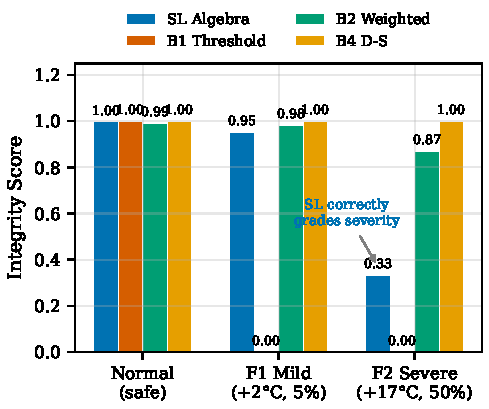
\includegraphics[width=\columnwidth]{figures/fig2_severity_discrimination.pdf}
\caption{Severity discrimination for insulin. The SL algebra correctly
grades mild ($P(\omega) = 0.95$) and severe ($P(\omega) = 0.33$)
excursions. B1 collapses both to 0.0 (binary). B4 Dempster-Shafer
produces 1.0 for all conditions, including severe failure.}
\label{fig:severity}
\end{figure}

\begin{figure}[t]
\centering
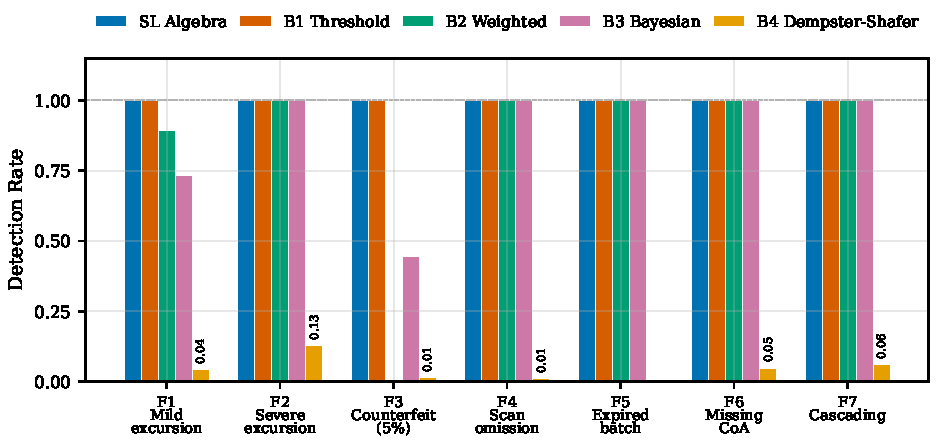
\includegraphics[width=\columnwidth]{figures/fig1_detection_rates.pdf}
\caption{Detection rates across seven failure scenarios (averaged over
three product categories). The SL algebra achieves DR=1.000 on every
scenario. B4 Dempster-Shafer fails to detect any scenario above 13\%.}
\label{fig:detection}
\end{figure}

\subsection{Severity Ranking}

We define a ground-truth severity ordering based on physical impact
(Normal $<$ F6 $<$ F4 $<$ F3 $<$ F5 $<$ F1 $<$ F7 $<$ F2) and compute
Spearman rank correlation between each method's mean scores and this
ordering. On insulin and mRNA the SL algebra achieves $\rho = 0.976$
($p = 3.3 \times 10^{-5}$); on amoxicillin it achieves $\rho = 0.786$
($p = 0.021$) under this ordering and $\rho = 0.976$ under a
product-specific ordering, fixed before recomputation, that ranks the
mild excursion below counterfeit and short dating for a room-temperature
tablet. In every case the SL algebra is the only method with a
statistically significant result. B1 ($\rho = 0.577$, $p = 0.134$), B2
($\rho = 0.431$, $p = 0.286$), and B3 ($\rho = 0.619$, $p = 0.102$) all
fail the $p < 0.05$ significance threshold, and B4's output is constant
(every score 1.000), so its rank correlation is undefined.
Fig.~\ref{fig:spearman} shows this comparison alongside
Shannon entropy of output distributions.

\begin{figure}[t]
\centering
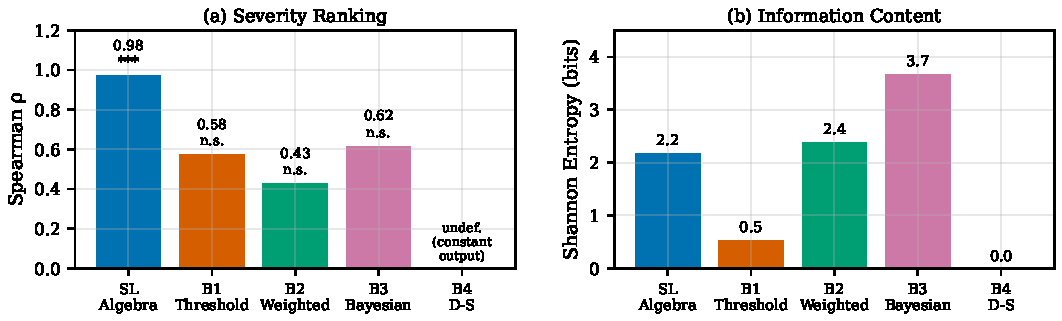
\includegraphics[width=\columnwidth]{figures/fig5_spearman_entropy.pdf}
\caption{(a) Spearman rank correlation with ground-truth severity
ordering. Only the SL algebra reaches statistical significance
(***~$p < 0.001$). (b) Shannon entropy of output distributions. B4
produces 0.0 bits (all scores identical at 1.0). B1 produces 0.5 bits
(near-binary). The SL algebra retains 2.2 bits of severity information.}
\label{fig:spearman}
\end{figure}

\subsection{Counterfeit Sensitivity}

We sweep the counterfeit infiltration rate in F3 from 1\% to 20\%
(Fig.~\ref{fig:counterfeit}). The SL algebra maintains DR=1.000 at all
levels, including 1\% infiltration: a single failed scan lowers the chain
score below the calibrated threshold because the noiseless Normal
distribution has a spread of 0.0001, and from 3\% the serialization
dimension's disbelief also exceeds the 0.02 per-dimension threshold. B1
passes exactly-1\% infiltration by construction
(its failure-rate limit is 1\%) and detects 2\% and above, so at this
level the algebra's edge over B1 is narrow and its edge over B2 and B3
wide; Section~\ref{sec:noise} shows that neither survives benign scan
errors at 100 packages per node. B2 requires at least 10\% infiltration before its
score crosses the adaptive threshold. B3 achieves majority detection
only above 5\%. B4 never exceeds DR=0.21 at any infiltration level and
shows no consistent trend, a consequence of evidence dilution in
Dempster's rule.

\begin{figure}[t]
\centering
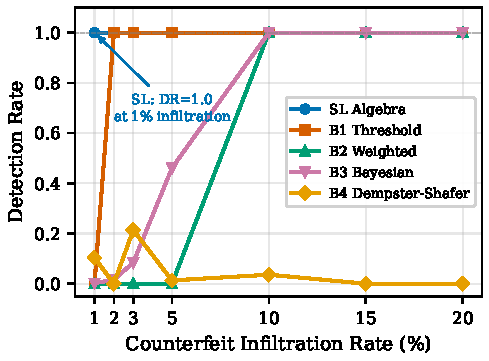
\includegraphics[width=\columnwidth]{figures/fig3_counterfeit_sweep.pdf}
\caption{Detection rate as a function of counterfeit infiltration rate.
The SL algebra detects 1\% counterfeiting with DR=1.000; B1 detects 2\%
and above; B2 requires 10$\times$ higher infiltration.}
\label{fig:counterfeit}
\end{figure}

\subsection{Ablation Analysis}

We perform five ablations, each modifying exactly one architectural
component (Fig.~\ref{fig:ablation}).

\textbf{A4 (Per-dimension detection)} is the only ablation that breaks
detection. Removing per-dimension monitoring and relying solely on the
chain-level score reduces F4 (scan omission) detection from DR=1.000 to
DR=0.297-0.369 across product categories. Scan omission manifests as
high uncertainty ($u \approx 0.80$) in the serialization dimension
without elevating disbelief, a pattern invisible to chain-level
aggregation but captured by per-dimension monitoring.

\textbf{A1 (Evidence type removal)} confirms clean one-to-one coupling
between evidence types and failure scenarios. Removing cold chain
evidence makes F1 and F2 scores indistinguishable from Normal. Removing
serialization evidence eliminates F3 and F4 discrimination. Each
evidence dimension is necessary for its matched failure type, validating
the multi-dimensional design.

\textbf{A2 (Fusion operator)} and \textbf{A3 (Propagation operator)}
show no impact on detection rates. Averaging fusion produces
$4.8\times$ higher uncertainty than cumulative fusion, and independent
node evaluation yields slightly higher Normal scores, but detection
remains at DR=1.000 for both. Their value is in uncertainty calibration
and semantic correctness, not detection capability.

\textbf{A5 (Evidence weights)} shows that product-specific weights
shift severity scores by 5-10\% on temperature failures but do not
affect detection rates.

\begin{figure}[t]
\centering
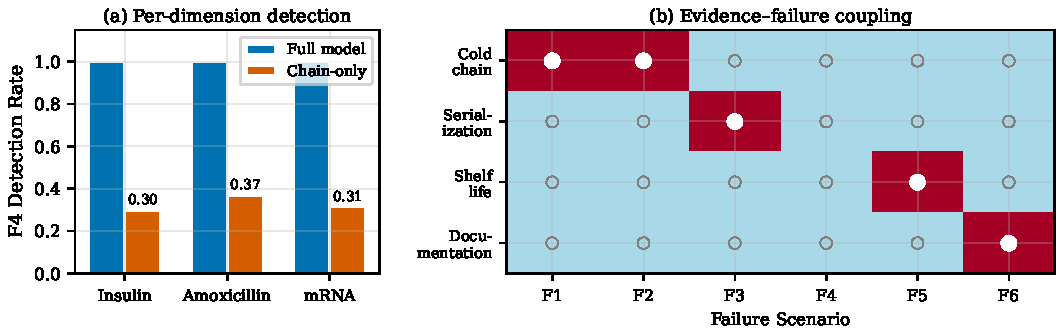
\includegraphics[width=\columnwidth]{figures/fig4_ablation.pdf}
\caption{(a) F4 detection with and without per-dimension monitoring.
Removal reduces DR from 1.0 to approximately 0.3. (b) Evidence-failure
coupling matrix. Filled circles mark where removing an evidence type
eliminates score discrimination for that failure scenario.}
\label{fig:ablation}
\end{figure}

\subsection{Dempster-Shafer Comparison}

B4 is the worst-performing method by every metric: DR below 0.13 on all
scenarios, AUC of 0.516 (near random), an undefined severity ranking
(constant output), and Shannon entropy of 0.0 bits (all scores are
identically 1.0). Two structural failures explain this result.

\textit{Conflict normalization.} Consider F2 (severe temperature
excursion), where 50\% of cold chain readings exceed the maximum by
17\textdegree C. Four evidence types (serialization, shelf life,
documentation, recall status) strongly support safety, producing mass
functions with $m(safe) > 0.6$. The cold chain mass function assigns
substantial mass to $m(compromised)$, but Dempster's rule normalizes the
conflict away ($K \approx 0.49$ at the failing node): the four agreeing
sources overwhelm the single dissenting source, and the pignistic
probability remains $BetP(safe) = 1.000$ (Table~\ref{tab:main_results}).
This is the normalization step that Zadeh's critique targets~\cite{zadeh1984},
reached here at moderate rather than total conflict. The SL algebra
assigns $P(\omega) = 0.332$ to the same scenario because cumulative fusion
preserves per-dimension disbelief rather than normalizing it away, and
the deduction operator propagates that disbelief causally through the
chain.

\textit{Evidence dilution.} With 25 mass functions combined via
Dempster's rule (5 evidence types at 5 nodes), $m(\Theta)$ approaches
zero exponentially and $m(safe)$ dominates. A failure signal in one of
25 sources has negligible impact on the combined result. Our
implementation combines the five evidence masses at each node and then
the five node masses; because Dempster's rule is associative, this
hierarchical grouping and a flat 25-source combination yield the same
mass function (verified to $10^{-15}$ on 25{,}000 simulated chains), so
no grouping can rescue the baseline. Dilution is structural: Dempster's
rule is designed for combining a small number of independent sources,
and it has no counterpart to the causal conditional through which our
deduction operator (J\o sang \S9.4) propagates upstream compromise.

\subsection{Operational Noise, Sensitivity, Fusion}
\label{sec:noise}

The Normal regime above contains no benign scan failures and no
out-of-range readings. We therefore add, at every node, benign scan
failures (0.5\% and 1\%), short temperature blips on 2\% and 5\% of
readings (up to 1 and 2\textdegree C), logger dropout (coverage down to
0.85 and 0.70) and late routine documents (5\% and 10\%), recalibrate
every method on 20{,}000 noisy Normal trials with the 1\% budget split
across its criteria (for the SL algebra: one disbelief and one
uncertainty threshold per evidence type, plus chain score and chain
uncertainty), and evaluate out of sample. Fixed rules fail at once: B1
as deployed, and the SL algebra with the fixed thresholds of
Section~III, flag nearly every clean chain (FPR 0.98 to 1.00).
Calibrated per evidence type, the SL algebra holds FPR at 0.001 to 0.009
and detects F2, F4, F5, F6 and F7 at 1.000 in both regimes, where B2
loses F6 (DR 0.06 to 0.10) and B3 detects it at 0.47 to 0.91. The subtle
failures are limited by evidence volume: with 100 packages and 100
readings per node, 5\% counterfeit is detected at 1.000 under moderate
noise but not under heavy noise, and the +2\textdegree C excursion is
not separable from blips at either level; with 1000 observations per
node both are detected (F3 at 1.000, F1 at 1.000 and 0.939). A rule
system re-tuned to the same noise matches this detection almost exactly,
so under noise, as in the clean regime, the algebra's advantage lies in
the graded score, the explicit uncertainty and node localization rather
than in the binary flag. The severity ordering remains significant at
1000 observations under moderate noise ($\rho = 0.762$, $p = 0.028$) but
not at 100.

Varying the formation parameters one at a time (conditional disbelief
0.8 to 1.0, critical-document weight 1 to 5, shelf-life scale 5 to 20,
prior weight 1 to 4, base rates, severity cap 2 to 10) leaves DR, LA and
FPR unchanged in every setting but one: a prior weight of 4 lifts the
documentation dimension's baseline uncertainty across the fixed 0.50
threshold on two products (FPR 1.000), one more reason per-dimension
thresholds must be calibrated; $\rho$ on insulin stays between 0.952
and 0.976 throughout. The five evidence types are independent
observation processes in our simulator ($|r| \le 0.013$ between their
disbelief values under noise). Compound failures whose root cause spans
two types at one node (counterfeit with a missing certificate, an
excursion on a short-dated batch, unscanned packages with late
paperwork) are detected and localized at 1.000 under cumulative and
under averaging fusion, score below their worse component in every
paired trial, and the two operators agree on the ordering
($\rho \ge 0.99$), averaging fusion carrying 4.7 times the uncertainty.

%===================================================================
\section{Discussion}
%===================================================================

\textbf{Clinical implications.} The graded integrity score gives
dispensing pharmacists actionable information beyond a binary flag. A
score of $P(\omega) = 0.95$ with low uncertainty suggests a minor
concern warranting monitoring, while $P(\omega) = 0.33$ signals a
likely compromise requiring quarantine. The per-dimension breakdown
identifies \textit{which} evidence type triggered the concern and at
\textit{which} node, enabling targeted investigation rather than
wholesale rejection. For the pharmacist this turns accept-or-reject into
a graded decision: a batch scored 0.95 with low uncertainty is dispensed
with a monitoring note, a batch scored 0.33 is quarantined, and a batch
whose score is high but whose serialization uncertainty is 0.8 is held
for verification rather than rejected, which matters because wholesale
rejection of batches with evidence gaps produces shortages that harm
patients as surely as compromised product does. Safety itself is not yet
a proposition of the algebra; the opinions concern batch integrity.
Patient safety can be modeled as a second proposition deduced from
integrity with product-specific conditionals, since a mild excursion
carries a different probability of clinical harm for insulin than for a
room-temperature tablet, and this uses the same operator set.

\textbf{Integration path.} The algebra operates on the same EPCIS event
data that Tatmeen already collects. By design, implementation requires
no change to the serialization infrastructure, only an assessment layer
consuming existing event streams; we have not yet run it against a live
system. The five evidence types map directly
to data elements mandated by Decree No.~73/2021 (Article~5) and the
Tatmeen technical guides~\cite{tatmeen_mfg_v5, tatmeen_logistics_v5}.

\textbf{Limitations.} Our evaluation is simulated, and the evidence
encodings and the failure injections rest on the same modeling
assumptions, so perfect detection in the noiseless regime is a
consistency check on the encoding rather than evidence of operational
performance; the rule-based baseline reaches the same detection there.
The severity orderings are author-defined; independent ranking by
pharmaceutical professionals with inter-rater agreement is in progress,
and the amoxicillin result shows that one global ordering does not fit
every product class. Per-dimension thresholds must be calibrated on the
deployment's Normal distribution, separately per evidence type; fixed
thresholds, ours included, fail under benign noise. Cumulative fusion
dilutes evidence types with few observations (a date, five documents) as
scan and temperature evidence accumulate, and averaging fusion does not
change this; per-type detection restores sensitivity, but the chain
score's ordering of low-count failures weakens with volume. Adversarial
manipulation, delayed reporting and conflicting records were not
evaluated; temporal decay (J\o sang \S16.2.2) is implemented but
inactive; and the simulation covers a single linear path, leaving the
multi-path fusion we have implemented unevaluated.

\textbf{Generalization.} While grounded in Tatmeen, the algebra applies
to any serialized pharmaceutical supply chain. The evidence taxonomy
(E1-E5) maps to DSCSA and EU FMD data elements with minor
adjustments to regulatory thresholds and document requirements. No
single ontology covers pharmaceutical supply-chain integrity, but the
vocabulary the algebra needs already exists in GS1 EPCIS 2.0 and its
Core Business Vocabulary~\cite{gs1epcis2022, gs1cbv2022}, which define
custody events, dispositions such as recalled or expired, and sensor
readings such as temperature, in JSON-LD, and are adopted as ISO/IEC
19987 and 19988. Because EPCIS 2.0 events are linked data, an SL opinion
(belief, disbelief, uncertainty, base rate) can be attached to an event
or to the batch it describes as a small annotation, which is how our
implementation stores opinions; aligning the algebra with these
vocabularies is a matter of naming the five evidence types with their
CBV terms, not of changing the algebra.

%===================================================================
\section{Conclusion}
%===================================================================

We presented a drug integrity algebra that replaces binary pass/fail
pharmaceutical supply chain assessment with graded, uncertainty-aware
integrity scores. Built on J\o sang's Subjective Logic and grounded in
the UAE Tatmeen system, the algebra matches the rule-based baseline on
detection and localization across seven failure scenarios while
providing the only statistically significant severity ranking among five
comparison methods and an explicit uncertainty that localizes the
affected evidence type and node. Under benign operational noise,
thresholds calibrated per evidence type hold a 1\% false-alarm target,
and detection of subtle failures scales with evidence volume.
Per-dimension opinion monitoring is the critical architectural
component, enabling detection of evidence gaps that chain-level scores
miss. The Dempster-Shafer baseline demonstrates that the closest
theoretical alternative produces zero information content in this
evaluation due to evidence dilution and conflict normalization. The
algebra is designed to consume the EPCIS event data that mandated
serialization systems already produce; its operational compatibility
remains to be demonstrated on live data.

%===================================================================
% REFERENCES
%===================================================================

\bibliographystyle{IEEEtran}
\bibliography{references}

\end{document}
